% !TEX encoding = UTF-8
% !TEX program = lualatex
\documentclass[10pt,letterpaper]{article}
\usepackage{cite}

\usepackage{style/arxiv}

\usepackage[T1]{fontenc}    % use 8-bit T1 fonts
\usepackage{url}            % simple URL typesetting
\usepackage{amsfonts}       % blackboard math symbols
\usepackage{amsmath}
\usepackage{csquotes}
\usepackage{tikz}

% define common tikz pictures for position representations
%\documentclass{article}
%\usepackage{tikz}
\tikzset {
    shape kanjiframe/.style= {
        draw,
        fill=white,
        ultra thick,
    }
}

\def\defkanjipos#1#2 {
    \tikzset {
        #1/.pic= { % first parameter defines the pic name
            code={
            \begin{scope}[transparency group, every path/.style={pic actions}]
                \pgftransformscale{0.5}
                \draw[pic actions, rounded corners=1pt, shape kanjiframe] (0,0) rectangle (1,1);
                #2 % second parameter is the code
            \end{scope}
            }
        }
    }
}

\defkanjipos{all}{
    \fill (0,0) rectangle (1,1);
}

\defkanjipos{top}{
    \fill (0,1) rectangle (1,0.5);
}

\defkanjipos{bottom}{
    \fill (0,0) rectangle (1,0.5);
}

\defkanjipos{left}{
    \fill (0,0) rectangle (0.5,1);
}

\defkanjipos{right}{
    \fill (0.5,0) rectangle (1,1);
}

\defkanjipos{kamae}{
    \fill (0,0) rectangle (1/3,1);
    \fill (2/3,0) rectangle ++(1/3,1);
    \fill (0,0) rectangle (1,1/3);
    \fill (0,2/3) rectangle ++(1,1/3);
}

\defkanjipos{tare}{
    \fill (0,0) rectangle (1/3,1);
    \fill (0,1) rectangle (1,2/3);
}

\defkanjipos{nyou}{
    \fill (0,0) rectangle (1/3,1);
    \fill (0,1/3) rectangle (1,0);
}

\defkanjipos{none}{}

%\begin{document}
%    \begin{tikzpicture}
%        \path (0,0) pic {top};
%        \path (0,-1) pic {kamae};
%        \path (0,-2) pic {left};
%    \end{tikzpicture}
%\end{document}

% tikz/pgf declarations
\usetikzlibrary {3d, arrows.meta, backgrounds, bending, calc, decorations.pathmorphing, decorations.shapes, fadings, fit,  graphs, graphdrawing, patterns, positioning, shapes.multipart, shapes.geometric}
\usegdlibrary {force, trees}


\usepackage[pagebackref=true,breaklinks=true,colorlinks,bookmarks=false]{hyperref}

% UTF-8 font supporting CJK characters
\usepackage{luatexja-fontspec}

% potentially use Noto font family, but this requires additional install

% \setmainjfont{NotoSerifCJK-Bold}
% \setmainjfont[     % setmainfontでもいいような
%   BoldFont={NotoSerifCJK-Bold},
%   BoldSlantedFont={NotoSerifCJK-Bold},
%   AutoFakeSlant=0.2,
%   SlantedFeatures={FakeSlant=0.2},
%   BoldSlantedFeatures={FakeSlant=0.2}]
% {NotoSerifCJK-Medium}

\title{Bidirectional Attention for Offline CJK Character Recognition}
\author{Tom Fuller}
\begin{document}

\maketitle
\listoffigures

\section{Introduction}
Currently, character classification for Chinese, Japanese, and Korean (CJK) languages has been very limited. In real-time classification, results have since been improved from prior SVM implementations with convolutional neural networks (CNN). Although referred to here as "CJK" languages/characters the term is used as a collective for the logographic characters used in Hong Kong, Taiwan, and Vietnam in addition to the aforementioned countries. Prior research has generally treated each Chinese character as a whole, ignoring the internal two-dimensional structure within each character. The most recent state-of-the-art work has started to incorporate structure, but only achieves 40.82\% accuracy on unseen handwritten characters, despite 96.66\% accuracy in recall\cite{denseran}. For printed Chinese characters, methods using metadata (multi-typed attributes) pushes the zero-shot performance to 56.6\%\cite{multi-attribute-recognition}, but is unable to translate results to handwriting samples.

Online recognition has more success, and is popular in mobile computing devices\cite{online-handwriting}, seeing heavy use in input method editors (IME). However, their reliance on temporal data makes them ineffective in OCR, and causes failures for incorrect stroke order.

Despite the over 40,000 characters needed for complete modern day coverage in present day Chinese, existing research has been reliant on the 3,755 characters of GB2312-80's level-1 set and the CASIA handwriting dataset\cite{casia-handwriting-db}. These characters form the "base set" needed for general literacy of Chinese. For Japanese, a set of 2,136 characters for basic literacy, the \textit{jōyō kanji}, is published by the Japanese Ministry of Education.

In other computer vision classification tasks, recognition across over 9,000 classes has been achieved, in the YOLOv2 architecture\cite{yolo}. It is unsurprising that the handwriting recognition approaches in similar architectures all boast recognition rates of slightly over 96\% for the 3,755 class size. The top three approaches are based on GoogLeNet \cite{hccr-googlenet}, ResNet \cite{multi-attribute-recognition}, and DenseNet \cite{denseran}.

The poor performance on characters landing outside of the level-1 metric is a problem that has not yet been solved. The current state-of-the-art method in both zero-shot and recall, DenseRAN\cite{denseran}, utilizes attention, but can fail easily if the wrong path in attention is taken. Thus, the intuition of this proposal is that a bidirectional and hierarchical attention mechanism is necessary within the Chinese, and by extension, CJK character classification task.
Bidirectional graph traversal allows for an efficient and correct encoding sequence of characters to be built. This intuition serves as the basis of the structure necessary to achieve performance in the zero-shot case, as well as recognition across the over 40,000 classes of Chinese logographic characters of modern use.


\section{CJK Character Structure}
While it has been stated that filters of smaller size are not suitable to recognize the complex relationships between Chinese strokes in convolutional architectures\cite{conv-chinese-character-synthesis}, this is overlooking fundamental hierarchies and geometric properties of logographic drawings.

Many approaches have focused on a specific language or script, for example Chinese\cite{online-ch}, Japanese\cite{online-ja}, or Korean\cite{offline-kr}. However, the structure can be generalized across CJK characters. In order to classify unseen characters, or a large number of characters, the intuition is that an approach leveraging these similarities be taken.

\subsection{Phono-semantic Compound Structure of Chinese characters}

Similar to the tree structure created by hyponyms and hypernyms of language which are captured within WordNet \cite{wordnet}, there exists a phono-semantic compound structure within many individual Chinese characters. Recent research on native Chinese speakers has shown the Stroop effect to occur, delaying recognition if misrepresented \cite{cjk-stroop}, indicating that the character recognition pathway within humans relies on these compounds. By decomposing compound ideographs into their constituent radicals, a graph can be created similar to the morphological decomposition and semantic field relationships within English. As over 80\% of the Chinese characters have been found to have this relationship \cite{compound-ideographs}. The intuition is that this structure is critical to obtaining fast character recall, creating a meaningful attention mechanism, and increasing performance in zero-shot classification.

\begin{figure}[h]
    \begin{center}
        \tikz[
        every shadow/.style={opacity=0.8,fill=blue!50!black},
        every pin/.style={font=\footnotesize}] {

            % Plant
            \node[shape=semicircle,shape border rotate=180, fill=cyan!20, inner sep=0.535cm] at (0, .95) {};
            \node[name=plant,circle split,very thick,pin=90:$semantic$,draw] at (0, 1.5) {\Huge 艹\nodepart{lower} plant};

            % Harvest
            \node[shape=semicircle,shape border rotate=180, fill=red!20, inner sep=0.575cm] at (0, -2.05) {};
            \node[name=harvest,set=component,circle split,very thick,pin=270:$phonetic$,draw] at (0, -1.5) {\Huge 采\nodepart{lower} harvest};

            % Claw
            \node[shape=semicircle,shape border rotate=180, fill=magenta!20, inner sep=0.535cm] at (-4.5, .95) {};
            \node[name=claw,circle split,very thick,draw] at (-4.5, 1.5) {\Huge ⺤\nodepart{lower} claw};

            % Tree
            \node[shape=semicircle,shape border rotate=180, fill=yellow!20, inner sep=0.575cm] at (-4.5, -2.05) {};
            \node[name=tree,circle split,very thick,draw] at (-4.5, -1.5) {\Huge 木\nodepart{lower} tree};

            % Vegetable
            \node[shape=semicircle,shape border rotate=180, fill=black!10, inner sep=0.575cm] at (4.5, -.575) {};
            \node[name=c,circle split,pin=90:$compound$,draw,very thick, double distance=2pt] at (4.5, 0) {\Huge 菜\nodepart{lower} vegetable};

            \begin{scope}[line width=2pt, arrows={-Stealth[length=10pt,inset=2pt]}]
               \draw (harvest) -> (c);
               \draw (plant) -> (c);
               \draw (claw) -> (harvest);
               \draw (tree) -> (harvest);
            \end{scope}
        }
        \caption[The Phono-semantic Relationship]{The phono-semantic relationship within the compound character, 菜 or \textit{vegetable}. The semantic component is a linguistic \textit{determinative}, providing the compound with elemental context. The phonetic component is semantically relevant here. Combined as \textit{"harvested plant"} for the character meaning \textit{vegetable}.}
        \label{fig:figure1}
    \end{center}
\end{figure}

\subsection{Kangxi Radical Position Encodings}

Kangxi radicals are the 214 radicals/roots comprising the compound characters of Chinese characters in CJK languages. As there are much fewer roots than possible constituents, positional encoding serves as a meta-feature necessary for classification beyond any base set.

In the Japanese encoding system, constituents are split into seven groups. These are \textit{top}, \textit{bottom}, \textit{left}, \textit{right}, \textit{kamae} (かまえ), \textit{tare} (たれ), and \textit{nyou} (にょう). The last three do not have equivalent words in English, but roughly translate to "enclosure", "hang down", and "wrap around bottom" respectively. The remaining case is for radicals themselves, which do not have a position. Totaling to a feature vector of size 8.

It is worth noting that the \textit{kamae} group represented by $\tikz\pic[color=gray, scale=0.6] at (0, -5pt) {kamae};$ in Figure \ref{fig:positions} is actually a grouping of positions that enclose another, but are less common than \textit{tare} or \textit{nyou}, and do not have a specific group. For example, 医 consists of \textit{kamae} radical 匚 enclosing 矢. The radical 匚 does not have an explicit stroke closing right side, although it can be thought of as being closed by deliberately missing stroke, differentiating it from 囗. Similarly, the radical 凵 is enclosed by a missing stroke on the top.

\begin{figure*}[t]
    \begin{center}
        \tikzset {
    shape kanjiframe/.style= {
        color=black!40,
        draw,
        fill=white,
        ultra thick,
    }
}

\def\defkanjipos#1#2 {
    \tikzset {
        #1/.pic = {
            \begin{scope}[every path/.style={color=black!40}]
            \pgftransformscale{0.5}
            \draw[rounded corners=1pt, shape kanjiframe] (0,0) rectangle (1,1);
            #2
            \end{scope}
            % \fill[fill=black!40] (0,0) rectangle ++(0.25, 0.5);
        }
    }
}

\defkanjipos{all}{
    \fill (0,0) rectangle (1,1);
}

\defkanjipos{top}{
    \fill (0,1) rectangle (1,0.5);
}

\defkanjipos{bottom}{
    \fill (0,0) rectangle (1,0.5);
}

\defkanjipos{left}{
    \fill (0,0) rectangle (0.5,1);
}

\defkanjipos{right}{
    \fill (0.5,0) rectangle (1,1);
}

\defkanjipos{kamae}{
    \fill (0,0) rectangle (1/3,1);
    \fill (2/3,0) rectangle ++(1/3,1);
    \fill (0,0) rectangle (1,1/3);
    \fill (0,2/3) rectangle ++(1,1/3);
}

\defkanjipos{tare}{
    \fill (0,0) rectangle (1/3,1);
    \fill (0,1) rectangle (1,2/3);
}

\defkanjipos{nyou}{
    \fill (0,0) rectangle (1/3,1);
    \fill (0,1/3) rectangle (1,0);
}

\defkanjipos{none}{}

\tikz {
    \foreach \x / \name in {0/top,1/bottom,2/left,3/right,4/kamae,5/tare,6/nyou,7/all} {
        \node at (0.25+\x,0.7) {\x};
        \pic at (\x,0) {\name};
    }
}

        \caption[Constituent Radical Positions]{The different positions of radicals within a CJK character. The encoded position uses 3 only bits. \newline From left to right: \(top\), \(bottom\), \(left\), \(right\), \(kamae\), \(tare\), \(nyou\), \(radical\)}
        \label{fig:positions}
    \end{center}
\end{figure*}

\subsection{Han Unification \& Unicode Ideographic Description Sequences}

To simplify similar character representations across Chinese (\textit{hanzi}), Japanese (\textit{kanji}), and Korean (\textit{hanja}) in the CJK languages, Unicode compresses similar representations into a single set of unified characters. This "Han unification" combines glyph variants by grapheme into a single code point within Unicode. The traditional Chinese glyph for "grass" uses four strokes in the radical (⺿), while simplified Chinese, Japanese, and Korean have three (⺾). The ⺿ and ⺾ characters both map to (U+8349, 草) and exist as variants. Due to the use as a radical, the four and three stroke variants contain separate encodings in the Unicode/CJK Radicals Supplement, allowing them to be rendered here.
Figure \ref{fig:han-unification} illustrates the effect on constituent radicals. The term \textit{ideograph} is used when referring to the set of glyph variants representing a common idea.

\begin{figure*}
    \begin{center}
        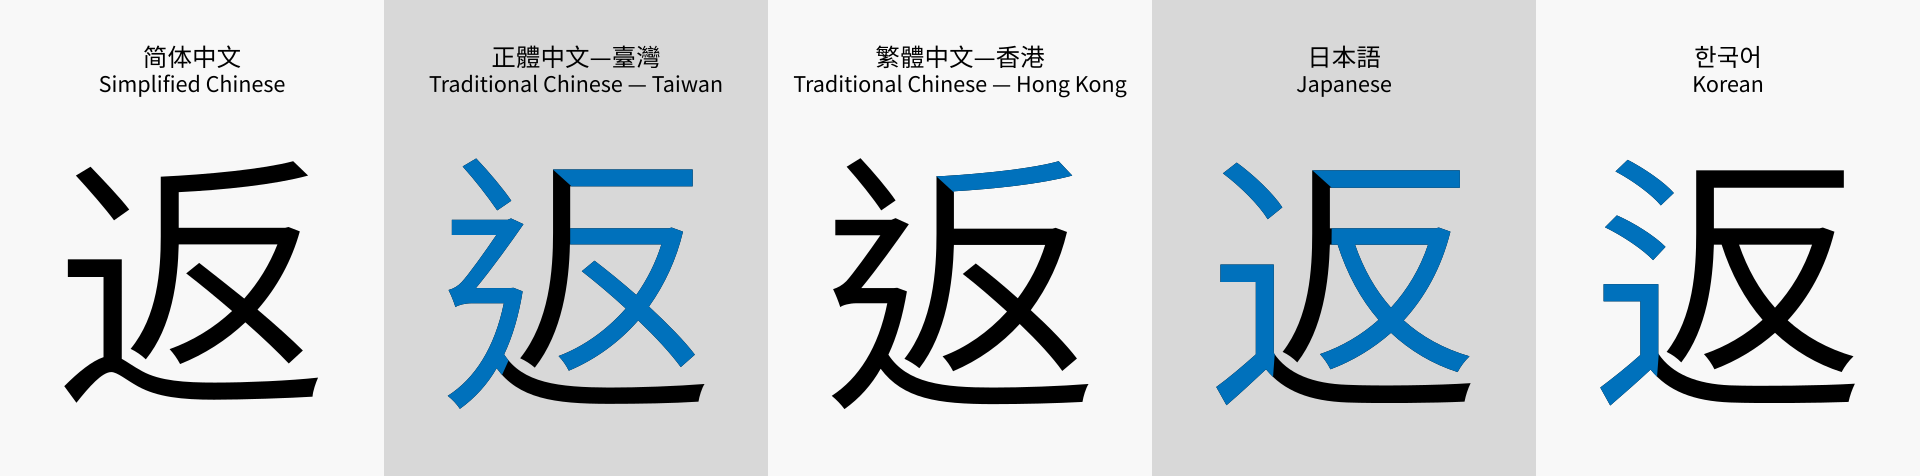
\includegraphics[width=1\textwidth]{figures/han_unification.png}
        \caption[Regional Character Variants]{Regional differences within the Unicode character (U+8FD4).
            Image in figure from Wikipedia\cite{wikipedia-han-unification}.}
        \label{fig:han-unification}
    \end{center}
\end{figure*}

Ideographic Description Sequences (IDS) in the Unicode standard\cite{unicode-ids} allows for any character to be encoded using logographic composition that is common across CJK characters. A representation sequence is shown in Figure \ref{fig:biang-ids}. Enocding sequences are not unique, and have a many-to-one relationship. The large quantity of strokes in the character \textit{biáng} in Figure \ref{fig:biang} illustrates that despite variations in constituents, a core set of ideographs determines the compound character meaning.

\begin{figure*}[h]
    \begin{center}
        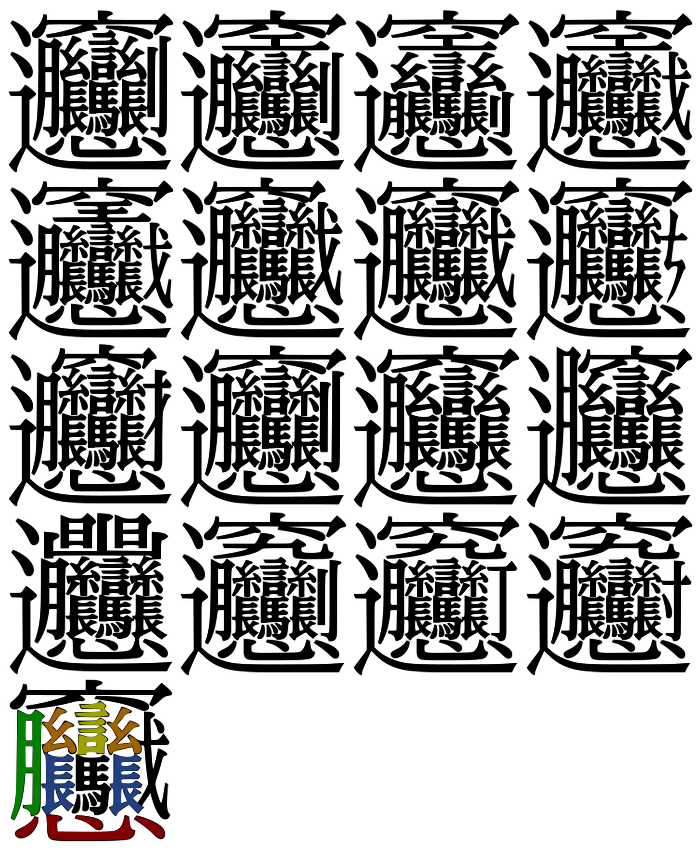
\includegraphics[width=0.3\textwidth]{figures/biang-variants.png}
        \caption[The 17 variants of \textit{biáng}]{The 17 variants of the character \textit{biáng}, a type of noodle. The last variant has constituents common across all variants colored to illustrate the core ideographs. \newline\textbf{These core constituents illustrate the intuition behind a bidirectional, multi-headed attention model.}}
        \label{fig:biang}
    \end{center}
\end{figure*}

\begin{figure*}[t]
    \begin{center}
        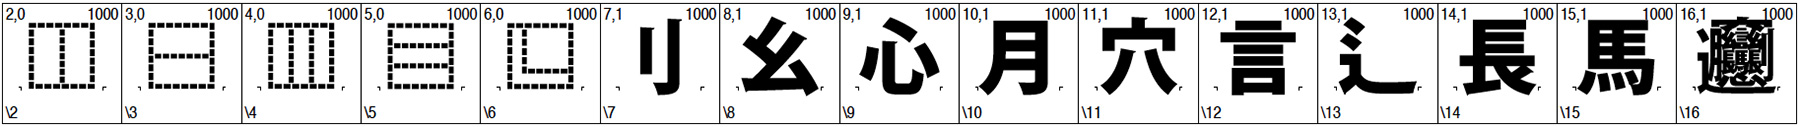
\includegraphics[width=1\textwidth]{figures/ids-biang.jpg}
        \caption[Unicode Ideographic Description Sequences]{An IDS of length 15 encoding the rendering of \textit{biáng} in OpenType. This sequence is just one capable of rendering \textit{biáng}, prior to it's inclusion in 2020\cite{unicode-ids}.
            Image in figure from Adobe \cite{adobe-ids}.}
        \label{fig:biang-ids}
    \end{center}
\end{figure*}


\section{Related Research}
\subsection{End-to-end Learning in Recurrent Attention Networks in Object Classification}
Within Chinese text recognition, end-to-end \cite{attention-hanzi} and bidirectional \cite{blstm-sentence-level} approaches have been used, but only as far as sentence level character segmentation. However recurrent attention has found use in image classification tasks \cite{residual-attention}, greatly reducing the number of connections and reducing error rates by comparison to ResNet. This has found it's way into DenseRAN \cite{denseran} at the character level, but does not consider the nested hierarchical nature of characters within the compounds.

\subsection{BERT - Deep Bidirectional Transformers}
Natural language processing has reached new heights with the novel approach of pre-trained bidirectional transformers in BERT\cite{bert}. While the concept of bi-directional attention is applied to the sentence level, I think the classic internet meme can illustrate the idea:

\begin{displayquote}
    \textit{Aoccdrnig to a rscheearch at Cmabrigde Uinervtisy, it deosn't mttaer in waht oredr the ltteers in a wrod are, the olny iprmoetnt tihng is taht the frist and lsat ltteer be at the rghit pclae. The rset can be a toatl mses and you can sitll raed it wouthit porbelm. Tihs is bcuseae the huamn mnid deos not raed ervey lteter by istlef, but the wrod as a wlohe.}
\end{displayquote}

Although the statement itself is not exactly true\cite{meme-text}, typoglycemic text demonstrates that the human brain is not actually processing the entirety of a word when reading quickly. Since the "shape" of the word is important, when parsing the word between two space delimiters, the brain notes key features at the first and last position, and works it's way inwards until it arrives at what it has considerable confidence is the word.

The application of pre-training transformers in BERT has been demonstrated in sentence-level tasks, and fine tuning at the token level. This has been done using a "masked language model" (MLM) as the pre-training objective for the encoder. By answering the question of "Which characters need to appear before the others" in a string of text, the ability to preserve semantic recall despite fluctuations in character sequence is made possible. Within NLP translation problems, this is the segmentation and reordering of the constituent concepts within a sentence.

When the decoder is then presented the encoded sequence, it is able to decode the concept sequences back to a readable format in the desired translation language.

\section{Proposed Architecture}
The problem of CJK character classification can be simplified by utilizing the structure within the characters. In order to tackle the handwritten recognition task effectively, we must simplify the problem. The approach outlined here is designed with goals of future extensibility through transfer learning. Each section describes a module that can be individually trained to achieve the end goal of offline CJK character recognition.

\subsection{Observe - Convolutional Handwriting Classifier}
The input must break the handwritten character into the constituent radicals that compose it. This task is similar to the object detection and classification problem. When performing detection in regions within a handwritten CJK character, the end goal is to group strokes belonging to each component within a compound character at the current depth. This can be performed on multiple feature grids by the multi-headed attention, providing resolution granularity during constituent observation. For an input, the network will return a feature vector of up to \(n\) constituents, $\vec{c}_n = <\vec{O}_0, \vec{O}_1, ... \vec{O}_{n-1}>$ at the current depth. The tuple $\vec{O}_n = (p_n,r_n)$ is the observed constituent at the current level, containing a position and radical encoding respectively.

The radical result, $r_n$ will be marked by \textbf{?} if the constituent is unrecognized, signaling to the Transformer that additional depth is needed in a particular region to achieve tokenization by the Encoder.

\subsection{Encode - Attention Based Character Tokenization}
The second network structure is the first half of a Transformer, prevalent in linguistic models of natural language processing\cite{transformers}. The Encoder uses the Observer network as a means of classification to tokenize a character into a sequence of embeddings. The embedding sequence leads to higher order classification at the Unicode character level, additionally driving the encoder-decoder attention.

Following the bidirectional attention mechanism of the Transformers as seen in BERT \cite{bert}, attention can be given areas for use by the Observer network. While the linguistic case is unidimensional over a series in text, the lexicographic case mandates two dimensions to span the character space as shown in Figure \ref{fig:attention} and \ref{fig:encoder}.

% figure of observations
\begin{figure*}[h]
    \begin{center}
        \definecolor{bluee}{HTML}{0022ff}
\definecolor{orangee}{RGB}{233,127,2}
\definecolor{yellowe}{RGB}{208,162,0}
\definecolor{rede}{HTML}{ff2200}
\definecolor{greene}{RGB}{138,155,15}

\definecolor{metac}{RGB}{56,62,64}
\definecolor{dkbluee}{RGB}{0,62,114}

%\begin{document}
\begin{tikzpicture}

    % input rectangle
    \draw (0,0) node[scale=5, anchor=center, color=black!70] {学};
	\node[color=greene, rectangle, draw, thick, minimum width=5em, minimum height=5em] (input) at (0, 0) {};


    \node[color=bluee, rectangle, draw, thick, minimum width=4.55em, minimum height=3em] (A) at (0, -0.75em) {};
    \node[color=orangee, rectangle, draw, thick, minimum width=4.725em, minimum height=2em] (B) at (0, 1.3em) {};

    \node[color=yellowe, rectangle, draw, dashed, thick, minimum width=4.6em, minimum height=1.1em] (C) at (0, 0.9em) {};
    \node[color=rede, rectangle, draw, dashed, thick, minimum width=3.65em, minimum height=1em] (D) at (0, 1.7em) {};


	\node[color=greene!60!black, below=0em of input] (l1) {\emph{input}};

    \begin{scope}[minimum width=4em]
        \fontsize{16}{16}
    	\node[dkbluee, rectangle, draw, above right=-1.5em and 3em of input, thick]  (Ob) {${\vec{o}_{\tikz\pic[scale=0.5,color=dkbluee] {top};{\textbf{?}}}}$};

    	\node[dkbluee, rectangle, draw, above=0em of Ob, thick]  (Oa)  {${\vec{o}_{\tikz\pic[scale=0.5,color=dkbluee] {bottom};{\normalsize \textbf{子}}}}$};
    	\node[dkbluee, rectangle, draw, below=0em of Ob, thick]  (Oc)  {${\vec{o}_{\tikz\pic[scale=0.5,color=dkbluee] {top};{\normalsize \textbf{⺍}}}}$};
    	\node[dkbluee, rectangle, draw, below=0em of Oc,thick]  (Od)  {${\vec{o}_{\tikz\pic[scale=0.5,color=dkbluee] {bottom};{\normalsize \textbf{冖}}}}$};
    \end{scope}

    \node[dkbluee, left=0em of Oa] (la) {$\tikz{\pic[scale=0.75, color=bluee] at (0,0) {bottom};}$};
	\node[dkbluee, left=0em of Ob] (lb) {$\tikz{\pic[scale=0.75, color=orangee] at (0,0) {top};}$};
	\node[dkbluee, left=0em of Oc] (lc) {$\tikz{\pic[scale=0.75, color=rede] at (0,0) {top};}$};
	\node[dkbluee, left=0em of Od] (ld) {$\tikz{\pic[scale=0.75, color=yellowe] at (0,0) {bottom};}$};

	\node[dkbluee, below=0em of Od] (lr) {\emph{observations}};

    \draw[bluee,-stealth, thick] (A) -- (la);
	\draw[orangee,-stealth, thick] (B) -- (lb);
	\draw[rede,-stealth, thick, dashed] (C) -- (lc);
	\draw[yellowe,-stealth, thick, dashed] (D) -- (ld);

	\node[draw, dkbluee, thick, right=20em of input] (O) {
        $\tikz{
            \pic[scale=0.75, color=dkbluee] at (0,0) {bottom};
            \node at (0.3,0.175) {\textbf{子}};
            \pic[scale=0.75, color=dkbluee] at (.8,0) {top};
            \pic[scale=0.75, color=dkbluee] at (1.3,0) {top};
            \node at (1.6,0.175) {\textbf{⺍}};
            \pic[scale=0.75, color=dkbluee] at (2.1,0) {bottom};
            \node at (2.4,0.175) {\textbf{冖}};
        }$
    };
	\node[dkbluee, below=0em of O] {\emph{embedding sequence}};

	\draw[dkbluee, densely dashed, very thick] (Oa.north east) -- (O.north west);
	\draw[dkbluee, densely dashed, very thick] (Od.south east) -- (O.south west);

	\fill [opacity=0.2, dkbluee] (Oa.north east) -- (O.north west) -- (O.south west) -- (Od.south east) -- cycle;

	% invisible nodes for relationship arc drawings
	\node[right=14.75em of input, inner sep=0em] (dum1) {};
	\node[right=1.5em of Ob, inner sep=0em] (dum2) {};
	\node[right=1.5em of Oc, inner sep=0em] (dum3) {};

	\draw[dkbluee, densely dotted, very thick] (Oa.east) edge[bend left=60] (Ob.east);
	\draw[dkbluee, densely dotted, very thick] plot [smooth, tension=1.5] coordinates { (Oa.east) (dum2) (Oc.east)};
	\draw[dkbluee, densely dotted, very thick] plot [smooth, tension=1.5] coordinates { (Oa.east) (dum1) (Od.east)};
	\draw[dkbluee, densely dotted, very thick] (Ob.east) edge[bend left=60] (Oc.east);
	\draw[dkbluee, densely dotted, very thick] plot [smooth, tension=1.5] coordinates { (Ob.east) (dum3) (Od.east)};
	\draw[dkbluee, densely dotted, very thick] (Oc.east) edge[bend left=60] (Od.east);

	\node[metac,rectangle, thick, align=center, draw, below left=3em and -4em of Od, text width=13.5em] (Q) {\texttt{"What order of constituent logograms encodes this handwritten input?"}};
	\node[metac,below=0em of Q] (ql) {\emph{encoder network}};

	\path[metac,-stealth, dashed, thick] (Q.east) edge[bend right] (6.2, -0.7);

	\node[dkbluee] at (7, 0) (EN){\textbf{\emph{BERT}}};

\end{tikzpicture}
%\end{document}
        \caption[Embedding Sequence Generation]{The interactions of the Encoder network.
            The encoder uses it's attention to query the Observer for observations in a given region.
            The observations are used to create an embedding sequence for the Decoder.
            The attention mechanism is then driven in jointly by both the encoder and the decoder's processing of the token sequence. }
        \label{fig:encoder}
    \end{center}
\end{figure*}

The Encode network needs only to provide enough focus to obtain a sequence of encoded inputs capable of returning the correct Unicode character by the Decoder. This in practice makes execution time much faster than the $O(n^2)$ theoretical bound of a Transformer. Time is saved by avoiding extraneous and potentially misleading classifications, which can be seen in Figure \ref{fig:biang}. Processing only core constituents solves the misalignment between focus order and stroke order. This also improves performance in characters with variants by resolving before attention is spent on the differing features.

\begin{figure*}
    \begin{center}
        \definecolor{col1}{RGB}{255,0,0}
\definecolor{col2}{RGB}{0,255,0}
\definecolor{col3}{RGB}{0,0,255}

\newcommand{\SinCos}[4]{
    \begin{scope}[xscale=(5/#2)/2]
        \draw[color=#1!80,#3] (-1,0) sin (0,1) cos (1,0) sin (2,-1) cos (3,0) sin (4,1) cos (5,0) sin (6,-1) cos (7,0) sin (8,1) cos (9,0) sin (10,-1) cos (11,0) sin (12,1);
        \draw[color=#1!80!black,densely dash dot,xshift=28pt,#4] (-1,0) sin (0,1) cos (1,0) sin (2,-1) cos (3,0) sin (4,1) cos (5,0) sin (6,-1) cos (7,0) sin (8,1) cos (9,0) sin (10,-1) cos (11,0) sin (12,1);

        %        absolute value version
        %        \draw[color=#1!60] (-1,0) sin (0,1) cos (1,0) sin (2,1) cos (3,0) sin (4,1) cos (5,0) sin (6,1) cos (7,0) sin (8,1) cos (9,0) sin (10,1) cos (11,0) sin (12,1);
        %        \draw[color=#1!60!black, xshift=28pt] (-1,0) sin (0,1) cos (1,0) sin (2,1) cos (3,0) sin (4,1) cos (5,0) sin (6,1) cos (7,0) sin (8,1) cos (9,0) sin (10,1) cos (11,0) sin (12,1);
    \end{scope}
}

\begin{tikzpicture}[scale=0.9]
\begin{scope}[xshift=-150pt]
%    \begin{scope}[yshift=40pt] % Draw grid lines
%        \draw[help lines, color=red, dashed] (0,0) grid (5,5);
%        \draw[help lines, color=green, dashed] (0,0) grid[step=5/3] (5,5);
%        \draw[help lines, color=blue, dashed] (0,0) grid[step=5/2] (5,5);
%    \end{scope}
%

    \begin{scope}[rotate around={-90:(6.4,0)}, yscale=-1]
        \draw[<-] (-0.2,0) -- (5.2,0) node[below,name=y] {$y$};
        \draw[<->] (0,-1.3) -- (0,1.3);
        \draw (0,1) -- (-0.1,1) node[above] {1};
        \draw (0,-1) -- (-0.1,-1) node[above] {-1};
        \draw[<->] (5,-1.3) -- (5,1.3);
        \clip (0,-1.1) rectangle (5,1.1);
        \SinCos{red}{5}{}{ultra thick}
        \SinCos{green}{3}{}{ultra thick}
        \SinCos{blue}{2}{}{ultra thick}
    \end{scope}

    \begin{scope}
        \draw[<-] (-0.2,0) -- (5.2,0) node[right,name=x] {$x$};
        \draw[<->] (0,-1.3) -- (0,1.3);
        \draw (0,1) -- (-0.1,1) node[left] {1};
        \draw (0,-1) -- (-0.1,-1) node[left] {-1};
        \draw[<->] (5,-1.3) -- (5,1.3);

        \clip (0,-1.1) rectangle (5,1.1);

        \SinCos{red}{5}{}{ultra thick}
        \SinCos{green}{3}{}{ultra thick}
        \SinCos{blue}{2}{ultra thick}{}
    \end{scope}

    \draw (6.4,0) circle (3.5em) node[name=circ, text width=3em]{};
    \draw[thick] (6.4,0) circle (1.5em) node[align=center,below]{};
    \node at ($(circ.south)-(0,1.5cm)$) {\textit{positional\ encoding}};
    \draw[thick] ($(circ.center)$) to [controls=+(90:1em)and +(90:1em)] ($(circ.center)-(1.5em,0)$);
    \draw[thick] ($(circ.center)$) to [controls=+(-90:1em)and +(-90:1em)] ($(circ.center)+(1.5em,0)$);

    % draw kanji
    \begin{scope}[line cap=round, line width=3, scale=0.5, yscale=-1.05, yshift=-395, yslant=0.25]
    \pgfkeys{/warp/.style={color=black}}
    \useasboundingbox(0,0) rectangle (38.1mm,38.1mm);

    %% Group layer1 --> top=True
    %% Group kvg:StrokePaths_05b66 --> top=False
    %% Group kvg:05b66 --> top=False
    %% Group kvg:05b66-g1 --> top=False
    %% Group kvg:05b66-g2 --> top=False
    %% path id="kvg:05b66-s1"
    %% path spec="m 29.5,17.25 c 3.5,3 6.5,7.25 7.75,9.75"
    \draw[/warp] (29.5mm,17.2mm)
    .. controls ++(3.5mm,3.0mm) and ++(-1.2mm,-2.5mm) .. ++(7.8mm,9.8mm)
    ;
    %% path id="kvg:05b66-s2"
    %% path spec="m 49,12 c 1.25,2 4.75,8.25 5.25,11.5"
    \draw[/warp] (49.0mm,12.0mm)
    .. controls ++(1.2mm,2.0mm) and ++(-0.5mm,-3.2mm) .. ++(5.2mm,11.5mm)
    ;
    %% path id="kvg:05b66-s3"
    %% path spec="m 75,11 c 0.25,1.75 -0.12,2.75 -0.75,4.25 -1.29,3.1 -4.25,7.38 -6.5,9.75"
    \draw[/warp] (75.0mm,11.0mm)
    .. controls ++(0.2mm,1.8mm) and ++(0.6mm,-1.5mm) .. ++(-0.8mm,4.2mm)
    .. controls ++(-1.3mm,3.1mm) and ++(2.2mm,-2.4mm) .. ++(-6.5mm,9.8mm)
    ;
    %% Group kvg:05b66-g3 --> top=False
    %% path id="kvg:05b66-s4"
    %% path spec="M 21.25,33.75 C 21.13,38.5 19.25,46.25 17.5,50"
    \draw[/warp] (21.2mm,33.8mm)
    %%%% Warning: check controls
    .. controls (21.1mm,38.5mm) and (19.2mm,46.2mm) .. (17.5mm,50.0mm)
    ;
    %% path id="kvg:05b66-s5"
    %% path spec="m 23.5,36.5 c 17,-1.62 42.38,-5.5 60,-5.75 9.5,-0.13 4.12,5.12 0,9"
    \draw[/warp] (23.5mm,36.5mm)
    .. controls ++(17.0mm,-1.6mm) and ++(-17.6mm,0.2mm) .. ++(60.0mm,-5.8mm)
    .. controls ++(9.5mm,-0.1mm) and ++(4.1mm,-3.9mm) .. ++(0.0mm,9.0mm)
    ;
    %% Group kvg:05b66-g4 --> top=False
    %% path id="kvg:05b66-s6"
    %% path spec="m 37.25,46.5 c 1,0.25 3.75,0.25 5.5,-0.25 1.75,-0.5 18.25,-4 20,-4 1.75,0 2.75,0.75 1,2.25 C 62,46 54.5,53.5 53,54.75"
    \draw (37.2mm,46.5mm)
    .. controls ++(1.0mm,0.2mm) and ++(-1.8mm,0.5mm) .. ++(5.5mm,-0.2mm)
    .. controls ++(1.8mm,-0.5mm) and ++(-1.8mm,0.0mm) .. ++(20.0mm,-4.0mm)
    .. controls ++(1.8mm,0.0mm) and ++(1.8mm,-1.5mm) .. ++(1.0mm,2.2mm)
    %%%% Warning: check controls
    .. controls (62.0mm,46.0mm) and (54.5mm,53.5mm) .. (53.0mm,54.8mm)
    ;
    %% path id="kvg:05b66-s7"
    %% path spec="m 50.75,55.75 c 4,8.75 7.18,24.67 1.75,38 -2.75,6.75 -7.75,1.25 -9.75,-2"
    \draw[/warp] (50.8mm,55.8mm)
    .. controls ++(4.0mm,8.8mm) and ++(5.4mm,-13.3mm) .. ++(1.8mm,38.0mm)
    .. controls ++(-2.8mm,6.8mm) and ++(2.0mm,3.2mm) .. ++(-9.8mm,-2.0mm)
    ;
    %% path id="kvg:05b66-s8"
    %% path spec="m 15.75,67.75 c 1.75,1 4.64,1.36 7.5,1 15.88,-2 44.43,-6.25 61.37,-5.5 2.5,0.11 4.72,0.25 6.39,1"
    \draw[/warp] (15.8mm,67.8mm)
    .. controls ++(1.8mm,1.0mm) and ++(-2.9mm,0.4mm) .. ++(7.5mm,1.0mm)
    .. controls ++(15.9mm,-2.0mm) and ++(-16.9mm,-0.8mm) .. ++(61.4mm,-5.5mm)
    .. controls ++(2.5mm,0.1mm) and ++(-1.7mm,-0.8mm) .. ++(6.4mm,1.0mm)
    ;
\end{scope}

    % add selection grid
    \begin{scope}[transform shape, line cap=round,scale=0.5, yshift=80]

    %\draw[help lines] (10mm,10mm) grid (100mm,100mm);

    \def\wgrid{100mm}

    \draw[help lines, red, dashed, thick] (0mm,0mm) grid [step=\wgrid/5] (\wgrid,\wgrid);
    \draw[help lines, green!80!black, dashed, thick] (0mm,0mm) grid [step=\wgrid/3] (\wgrid,\wgrid);
    \draw[help lines, blue, dashed, thick] (0mm,0mm) grid [step=\wgrid/2] (\wgrid,\wgrid);
    \clip (0mm, 0mm) rectangle (\wgrid, \wgrid);

    \def\gx{1}
    \def\gy{2}
    \def\gxx{5}
    \def\bx{1}
    \def\by{0}
    \def\rx{1}
    \def\ry{1}
    \def\rwidth{3}
    \newcommand{\dr}{\wgrid/10}
    \newcommand{\dg}{\wgrid/6}
    \newcommand{\db}{\wgrid/4}

    \newcommand{\AttentionGrid}[2]{
        \node (blue) [rounded corners=1pt, #1=blue!90!black, minimum height=2*\db, minimum width=2*\db, #2] at (\db+\bx*\db,\db+\by*\db) {};
        \node (red) [rounded corners=1pt, #1=red!90!black, opacity=0.8, minimum height=2*\rwidth*\dr, minimum width=2*\rwidth*\dr, #2] at (\dr + \rx*\dr + \rx*\rwidth*\dr,\dr + \ry*\rwidth*\dr + \ry*\dr) {};
        \node (green) [rounded corners=1pt, #1=green!80!black, minimum height=2*\dg, minimum width=2*\dg, #2] at (\gx*\dg,\dg+\gy*\dg) {};

        \node (green2) [rounded corners=1pt, #1=green!80!black, minimum height=2*\dg, minimum width=2*\dg, #2] at (\gxx*\dg,\dg+\gy*\dg) {};
    }

    \begin{scope}[transparency group, fill opacity=0.55, draw opacity=1]
        \begin{scope}[blend group=screen]
            \AttentionGrid{fill}{}
        \end{scope}
    \end{scope}
    %
    \begin{scope}[transparency group, opacity=0.8, every node/.style={fill=none}]
        \AttentionGrid{ultra thick,draw,color}{remember picture}
    \end{scope}
\end{scope}

\end{scope}

\begin{scope}[yshift=0,xshift=0+175,on background layer]
    % Under Creative Commons Attribution licence 3.0
% (http://creativecommons.org/licences/by/3.0)
% Author: Tom Fuller
% Adapted from TikZ Cuboid Computation by: Florian Lesaint


%\definecolor{col1}{RGB}{255,0,0}
%\definecolor{col2}{RGB}{0,255,0}
%\definecolor{col3}{RGB}{0,0,255}


\newcommand{\generateRefPoints}[7]{
    % 1 = square width (-2cm)   = to be transformed by perspective computation
    % 2 = square height (-2cm)  = given position at 0
    % 3 = center_x (0)
    % 4 = center_y (0)
    % 5 = range (8cm)
    % 6 = above (1.5cm)
    % 7 = below (2cm)
    %
    % // todo: take array of lengths relative to prior
    % 1 = len1
    % 2 = len2
    % 3 = len3

    \pgfmathparse{#4+#2}    % center - height = underview
    \pgfmathresult \let\yunder\pgfmathresult;

    \pgfmathparse{#6+#4}    % center - height = overview
    \pgfmathresult \let\yabove\pgfmathresult;

    \pgfmathparse{#5-#3}    % center - width = base (positive)
    \pgfmathresult \let\px\pgfmathresult;

    \pgfmathparse{-#2}
    \pgfmathresult \let\ybelow\pgfmathresult;


    %    above = y_dist(a1 - p1); below = y_dist(a2 - p1)


    %    phi = atan(above/px)
    %    s*90 = 180 - 2*phi; solve for s
    %    x` = s * (above/below)
    %    y` = s * sin(phi)


    \pgfmathparse{atan2(\yabove,\px)}
    \pgfmathresult \let\phi\pgfmathresult;
    \pgfmathparse{(180 - 2*\phi)/90}    % obtain the side using law of sines, 90 degree angle avoids a sine call
    \pgfmathresult \let\side\pgfmathresult;

    % compute the new x from the above/below; simplified sin(90) = 1
    \pgfmathparse{\side * (\yabove / \ybelow)}
    \pgfmathresult \let\xprime\pgfmathresult;

    % TODO: FIX x-ratio by getting the ratio of the known height to the distance half way between P2
    % TODO: and then use as known side length for obtaining ratio to halfway to P1
    \pgfmathparse{#2/#1}
    \pgfmathresult \let\xratio\pgfmathresult;

    % now get a ratio to the perspective point from the relative x
    \pgfmathparse{(scalar(\px/1cm) + \xratio*\xprime)/scalar(\px/1cm)}  % TODO: devise a way to remove the units... cmon
    \pgfmathresult \let\ratio\pgfmathresult;


    %% Vanishing points for perspective handling
    \coordinate (P1) at (-#5, #6); % left vanishing point (To pick)
    \coordinate (P2) at (#5, #6);  % right vanishing point (To pick)

    %% (A1) and (A2) defines the 2 central points of the cuboid
    % TODO: use the parameters for center x and y
    \coordinate (A1) at (0em,0cm); % central top point (To pick)
    \coordinate (A2) at (0em,-#2); % central bottom point (To pick)

    % the picture always fits in half the range to make even
    \coordinate (X1) at ($(P2)!.5!(A1)$);
    \coordinate (X2) at ($(P2)!.5!(A2)$);

    %% (A3) to (A8) are computed given a unique parameter (or 2) .8
    % You can vary .8 from 0 to 1 to change perspective on left side
    \coordinate (A3) at ($(P1)!\ratio!(A2)$); % To pick for perspective
    \coordinate (A4) at ($(P1)!\ratio!(A1)$);

    % y prime is not needed, but is computed as such from law of sines
%    \pgfmathparse{\side * sin(\phi)}
%    \pgfmathresult \let\yprime\pgfmathresult;
%
%    % Draw debug point (needs yprime uncommented)
%    \draw[fill=black!80!transparent] (\xprime, \yprime) circle (2em) node[color=white] {\tiny \xratio};
}

% Generate the vanishing points for this concatenation
% TODO: clean up arguments for initial point generation
% TODO: factor out concatenated cube generation
\generateRefPoints{2cm}{2cm}{0}{0}{8cm}{1.5cm};

%%% Vanishing points for perspective handling
%\coordinate (P1) at (-8cm, 1.5cm); % left vanishing point (To pick)
%\coordinate (P2) at (8cm, 1.5cm);  % right vanishing point (To pick)
%
%%% (A1) and (A2) defines the 2 central points of the cuboid
%\coordinate (A1) at (0em,0cm); % central top point (To pick)
%\coordinate (A2) at (0em,-2cm); % central bottom point (To pick)
%
%\coordinate (X1) at ($(P2)!.5!(A1)$);
%\coordinate (X2) at ($(P2)!.5!(A2)$);
%
%% (A3) to (A8) are computed given a unique parameter (or 2) .8
% You can vary .8 from 0 to 1 to change perspective on left side
%\coordinate (A3) at ($(P1)!.8346!(A2)$); % To pick for perspective
%\coordinate (A4) at ($(P1)!.8346!(A1)$);

% You can vary .8 from 0 to 1 to change perspective on right side
\coordinate (A7) at ($(P2)!.9375!(A2)$);
\coordinate (A8) at ($(P2)!.9375!(A1)$);

%% Automatically compute the last 2 points with intersections
\coordinate (A5) at
(intersection cs: first line={(A8) -- (P1)},
   second line={(A4) -- (P2)});
\coordinate (A6) at
(intersection cs: first line={(A7) -- (P1)},
   second line={(A3) -- (P2)});


\coordinate (B1) at ($(P2)!.995!(A8)$);
\coordinate (B2) at ($(P2)!.995!(A7)$);

\coordinate (B3) at ($(P2)!.995!(A6)$);
\coordinate (B4) at ($(P2)!.995!(A5)$);

\coordinate (B7) at ($(P2)!.775!(A2)$);
\coordinate (B8) at ($(P2)!.775!(A1)$);


\coordinate (B5) at
  (intersection cs: first line={(B8) -- (P1)},
            second line={(A5) -- (P2)});

\coordinate (B6) at
  (intersection cs: first line={(B7) -- (P1)},
            second line={(A6) -- (P2)});



\coordinate (C1) at ($(P2)!.995!(B8)$);
\coordinate (C2) at ($(P2)!.995!(B7)$);

\coordinate (C3) at ($(P2)!.995!(B6)$);
\coordinate (C4) at ($(P2)!.995!(B5)$);

\coordinate (C7) at ($(P2)!.625!(B2)$);
\coordinate (C8) at ($(P2)!.625!(B1)$);


\coordinate (C5) at
(intersection cs: first line={(C8) -- (P1)},
second line={(B5) -- (P2)});

\coordinate (C6) at
(intersection cs: first line={(C7) -- (P1)},
second line={(B6) -- (P2)});

%%%%%%%%%%%%%%%%%%%%%%
%%%%%%%%%%%%%%%%%%%%%% Start filling

\fill[col1!70!black] (C2) -- (C3) -- (C6) -- (C7) -- cycle; % bottom face
\fill[col1!50] (C3) -- (C4) -- (C5) -- (C6) -- cycle;  % far left face
\fill[col1!30,opacity=0.5] (C5) -- (C6) -- (C7) -- (C8) -- cycle; % far right face
\draw[thick,dashed] (C5) -- (C6);
\draw[thick,dashed] (C3) -- (C6);
\draw[thick,dashed] (C7) -- (C6);
\fill[col1,opacity=0.7] (C1) -- (C8) -- (C7) -- (C2) -- cycle; % face 1
\node at (barycentric cs:C1=1,C8=1,C7=1,C2=1) {}; % \tiny c1};
\fill[col1,opacity=0.3] (C1) -- (C2) -- (C3) -- (C4) -- cycle; % c2
\fill[col1,opacity=0.7] (C1) -- (C4) -- (C5) -- (C8) -- cycle; % c5
\node (t1) [anchor=north] at (barycentric cs:C1=1,C4=1,C5=1,C8=1) {};
\draw[thick] (C1) -- (C2);
\draw[thick] (C3) -- (C4);
\draw[thick] (C7) -- (C8);
\draw[thick] (C1) -- (C4);
\draw[thick] (C1) -- (C8);
\draw[thick] (C2) -- (C3);
\draw[thick] (C2) -- (C7);
\draw[thick] (C4) -- (C5);
\draw[thick] (C8) -- (C5);

%\fill[green!70!black] (B2) -- (B3) -- (B6) -- (B7) -- cycle;
%\fill[green!50!black] (B3) -- (B4) -- (B5) -- (B6) -- cycle;
%\fill[green!30] (B5) -- (B6) -- (B7) -- (B8) -- cycle; % far face

\fill[col2!70!black] (B2) -- (B3) -- (B6) -- (B7) -- cycle;
\fill[col2!50] (B3) -- (B4) -- (B5) -- (B6) -- cycle;
\fill[col2!30,opacity=0.5] (B5) -- (B6) -- (B7) -- (B8) -- cycle; % far right face

\draw[thick,dashed] (B5) -- (B6);
\draw[thick,dashed] (B3) -- (B6);
\draw[thick,dashed] (B7) -- (B6);

\fill[col2,opacity=0.7] (B1) -- (B8) -- (B7) -- (B2) -- cycle; % face 1
\node at (barycentric cs:B1=1,B8=1,B7=1,B2=1) {}; % \tiny b1};

\fill[col2,opacity=0.3] (B1) -- (B2) -- (B3) -- (B4) -- cycle; % b2
%\node at (barycentric cs:B1=1,B2=1,B3=1,B4=1) {\tiny b2};

\fill[col2,opacity=0.7] (B1) -- (B4) -- (B5) -- (B8) -- cycle; % f5
\node (t2) [anchor=north] at (barycentric cs:B1=1,B4=1,B5=1,B8=1) {};


\draw[thick] (B1) -- (B2);
\draw[thick] (B3) -- (B4);
\draw[thick] (B7) -- (B8);
\draw[thick] (B1) -- (B4);
\draw[thick] (B1) -- (B8);
\draw[thick] (B2) -- (B3);
\draw[thick] (B2) -- (B7);
\draw[thick] (B4) -- (B5);
\draw[thick] (B8) -- (B5);

%%%
%%%

%% Possibly draw back faces
\fill[col3!70!black,opacity=0.7] (A2) -- (A3) -- (A6) -- (A7) -- cycle; % face 6
%\node at (barycentric cs:A2=1,A3=1,A6=1,A7=1) {\tiny f6};

\fill[col3!50!black,opacity=0.7] (A3) -- (A4) -- (A5) -- (A6) -- cycle; % face 3
%\node at (barycentric cs:A3=1,A4=1,A5=1,A6=1) {\tiny f3};

\fill[col3!30,opacity=0.5] (A5) -- (A6) -- (A7) -- (A8) -- cycle; % face 4
%\node at (barycentric cs:A5=1,A6=1,A7=1,A8=1) {\tiny f4};

\draw[thick,dashed] (A5) -- (A6);
\draw[thick,dashed] (A3) -- (A6);
\draw[thick,dashed] (A7) -- (A6);


%% Possibly draw front faces

\fill[col3,opacity=0.7] (A1) -- (A8) -- (A7) -- (A2) -- cycle; % face 1

\fill[col3!70!black,opacity=0.7] (A1) -- (A2) -- (A3) -- (A4) -- cycle; % f2

\fill[col3,opacity=0.7] (A1) -- (A4) -- (A5) -- (A8) -- cycle; % f5

\node at (barycentric cs:A1=1,A8=1,A7=1,A2=1) {};%\tiny a1};

\node at (barycentric cs:A1=1,A2=1,A3=1,A4=1) {};%\tiny a2};

\node (t3) [anchor=north] at (barycentric cs:A1=1,A4=1,A5=1,A8=1) {};

%% Possibly draw front lines
\draw[thick] (A1) -- (A2);
\draw[thick] (A3) -- (A4);
\draw[thick] (A7) -- (A8);
\draw[thick] (A1) -- (A4);
\draw[thick] (A1) -- (A8);
\draw[thick] (A2) -- (A3);
\draw[thick] (A2) -- (A7);
\draw[thick] (A4) -- (A5);
\draw[thick] (A8) -- (A5);

% Draw debug points
%\foreach \i in {1,2,...,8} {
%    \draw[fill=black] (A\i) circle (0.25em) node[color=white] {\tiny \i};
%}
%
%\draw[fill=black] (P1) circle (0.1em) node[below] {\tiny p1};
%\draw[fill=black] (P2) circle (0.1em) node[below] {\tiny p2};

\end{scope}

\begin{scope}[yshift=64,xshift=260,z={(10:10mm)},x={(165:10mm)}]
    \begin{scope}[canvas is zx plane at y=0, scale=1.125]

    % Draw the Kanji stroke on the grid
    \input{figures/kanji-learn-svg.tex}

    \input{figures/grid-selection.tex}
    \end{scope}

    \begin{scope}[canvas is zy plane at x=0]
        \node (head) at ($(blue.south)+(0.25,-0.25)$) [transform shape] {multi-head attention};
    \end{scope}

    \begin{scope}[z={(12.5:7mm)},canvas is zy plane at x=0]
        \node (conv) at ($(blue.south)+(0,-1.1)$) [transform shape] {{\footnotesize convolutional observation network}};
    \end{scope}

    \begin{scope}[z={(15:5mm)},canvas is zy plane at x=0]
        \draw[transform shape, ->] (head) -> (conv);
        \node (conc) at ($(blue.south)+(-1.5,-2)$) [transform shape] {concatenate};
    \end{scope}

\end{scope}
\begin{scope}[xshift=260,z={(26:10mm)},x={(165:15mm)}] %,y={(-155:10mm)}]
    \begin{scope}[canvas is zx plane at y=-200]
        \node at ($(B7.south)+(-0.5, -0.5)$) [transform shape] {encoder-decoder attention};
    \end{scope}
\end{scope}

\draw[->] (conv) -> (conc);

% TODO: ensure that these points exist on the concat-filters-3d
\begin{scope}[on background layer, out=-90,in=90,looseness=1.5, opacity=0.7]
    \draw[red!80!black, ultra thick, double distance=1pt] (red.mid) to (t1);
    \draw[green!80!black,ultra thick, double distance=1pt] (green.mid) to (t2);
    \draw[green!80!black,ultra thick, double distance=1pt] (green2.mid) to (t2);
    \draw[blue!80!black,ultra thick, double distance=1pt] (blue.mid) to (t3);
\end{scope}

\end{tikzpicture}

        \caption[Multi-head Positional Encoding of Transformer]{The positional encoding mechanism of the Transformers. On the left, input sinusoids are shown. The selected waves in bold are chosen arbitrarily from each sine and cosine pair. The waves of highest energy for a given input is selected to control the area of attention. On the right, the same attention selection for the three heads is shown being passed through the convolutional observer and concatenated. The concatenated result is then used by the Encoder and Decoder to determine future positions of attention.}
        \label{fig:attention}
    \end{center}
\end{figure*}

\subsection{Decode - Unicode Character Retrieval from Embedding Sequence}
The final portion of the network will process two encoded sequences in parallel, as part of the bidirectional approach seen in BERT\cite{bert}. By creating two regions of focus, the result can be reached faster, and potentially without using all the information. The main result from the decoder is in providing a single UTF-16 character (represented across a weighted probability vector of all Unicode CJK characters).

Since the decode network takes only a tokenized embedding sequence, the decoder can be trained quickly with ground truth data outside of the computer vision components. Fine tuning of Transformers in subsequent training sessions has been quite effective\cite{transformers}\cite{bert}. By training the fully connected output layers from the decoder, future questions can be answered, making this architecture extensible.

\subsection{Summary}
The Observer network will learn
\begin{itemize}
    \item "Are any CJK constituents located in this handwriting sample? Where?"
    \item "Is the constituent a known radical? should it be broken further?"
\end{itemize}
The Encode network will learn
\begin{itemize}
    \item "What does the position of one ideograph mean in relation to others?"
    \item "What region should get attention so a tokenized sequence can be given to the decoder?"
\end{itemize}
The Decode network will learn
\begin{itemize}
    \item "What Unicode CJK character does this sequence of radicals and positions represent?"
    \item "After what has been seen, what region should get attention next?"
\end{itemize}

The operational flow of the entire network is shown in Figure \ref{fig:use}.

\newpage
\newcommand\tab[1][1cm]{\hspace*{#1}}
\section{Overview}
\begin{figure*}[h]
    \begin{center}
        %\documentclass[crop, tikz]{standalone}
%\usepackage{tikz}
%\usepackage{amsmath}
%
%\usetikzlibrary{decorations.pathmorphing, positioning, backgrounds, arrows.meta, calc}

\definecolor{echoreg}{HTML}{ff4400}
\definecolor{echodrk}{HTML}{0044ff}

\tikzstyle{mynode} = [text=black, very thick,
    rectangle, inner sep=10pt, inner ysep=20pt]
\tikzstyle{fancytitle} =[text=black]


\tikzstyle{labelnode} = [text=black, very thick,
draw=none, font=\normalsize, outer sep=0pt]

\newcommand{\yslant}{0.5}
\newcommand{\xslant}{-0.6}

\begin{tikzpicture}[scale=0.58,every node/.style={minimum size=1cm},on grid]

	\node [mynode, scale=0.85] at (10.5, 0) (box){%
		\begin{minipage}{0.2\textwidth}

          \tikz[
              yshift=50,
              edge from parent path={(\tikzparentnode.south) -- (\tikzchildnode.north)},
              every child node/.style={color=black,scale=0.35,thick,outer sep=0pt,circle,minimum size=16pt,draw,column sep={1.5pt,between origins}},
              font=\Huge
          ] {

          % define the set of forward observed nodes
          \node (fA) [draw, thick, circle, scale=0.35, fill=echoreg!20] at (0,0) {A}; % 十 pin={0:\scriptsize{t}}
          \node (fB) [draw, thick, circle, scale=0.35, fill=echoreg!20] at (0,-1) {\textbf{?}};
          \node (fX) [draw, thin, circle, scale=0.35, fill=white] at (1,-1) {宀}; % 宀 (字)
          \pic [scale=0.9] at ($(fA.mid)-(0.225,0.155)$) {top};
          \node (fC) [draw, thick, circle, scale=0.35, fill=echoreg!40, double] at (0,-2) {C};
          \pic [scale=0.9] at ($(fC.mid)-(0.225,0.155)$) {top};
          \node (fD) [draw, dashed, thick, circle, scale=0.35, fill=white] at (1,-2) {D};
          \pic [scale=0.9] at ($(fD.mid)-(0.225,0.155)$) {bottom};

          % define the set of result nodes
          \begin{scope}[xshift=5,yshift=5,scale=1.1,
              every pin edge/.style={draw=none}]
              \node (rA) [draw, thick, circle, scale=0.35, fill=white, dashed] at (0,-4) {⺾}; % ⺾ (芥) 1st CUT [荐,菰 because bottom is compound, top is not]; also cuts 芥苓茶荅荼莟蒼蓉蔭蓼薈... after first observation without having to look at [top][bottom] to determine if it is 冖 or 𠆢. ⺾/𠆢 in this path is fully cut before observation of [top][top] because ALL possible bottom characters in the tree are not 子.

              \node (rB) [draw, thick, circle, scale=0.35, fill=white, pin={[pin distance=-15pt]below:\textsf{孛}}] at (1,-4) {十}; % 十 (孛/character)(學/school)
              \node (rC) [draw, thick, circle, scale=0.35, fill=echoreg!50!echodrk!50, double, pin={[name=p1,pin distance=-15pt]below:\textbf{\underline{学}}}] at (2,-4) {\textbf{⺍}}; % ⺍ (学/study)
              \node (rD) [draw, thick, circle, scale=0.35, fill=white, pin={[pin distance=-15pt]below:學}] at (3,-4) {𦥯}; % 𦥯 (學/school)
              \node[labelnode, above=-15pt, scale=1.15] at ($(p1.south)$) {\textbf{(f)}};
          \end{scope}
          % 學学孛字孕

%          \node (D) [draw, thick, circle, scale=0.35, fill=echoreg!40] at (2,-5) {D};

%  電子 (でんしゃ) means "electron" but literally translates to "electric child", 孛 combines "above" and "child"



          \begin{scope}[xshift=70]
              \node (bA) [draw, thick, circle, scale=0.35, fill=echodrk!20] at (0,0) {A};
              \node (bB) [draw, thick, circle, scale=0.35, fill=echodrk!20] at (0,-1) {\textbf{子}};
              \pic [scale=0.9] at ($(bA.mid)-(0.225,0.155)$) {bottom};
              \node (bC) [draw, thick, circle, scale=0.35, fill=echodrk!40] at (1,-1) {C};
              \pic [scale=0.9] at ($(bC.mid)-(0.225,0.155)$) {top};

              \node (bD) [draw, thick, circle, scale=0.35, fill=echodrk!40, double] at (0,-2) {D};
              \pic [scale=0.9] at ($(bD.mid)-(0.225,0.155)$) {top};

              \node (bE) [draw, thick, circle, scale=0.35, fill=white, dashed] at (1,-2) {E};
              \pic [scale=0.9] at ($(bE.mid)-(0.225,0.155)$) {bottom};
          \end{scope}

          \node[labelnode, scale=1.15] at ($(fD)!.5!(bD) - (0,15pt)$) {\textbf{(e)}};
          \draw[ultra thick] (fA) -- (fB);
          \draw[ultra thick] (fB) -- (fC);
          \draw[thin] (fA) -- (fX);
          \draw[densely dashed] (fB) -- (fD);

          \draw[ultra thick] (bA) -- (bB);
          \draw[ultra thick] (bB) -- (bC);
          \draw[ultra thick] (bC) -- (bD);
          \draw[densely dashed] (bC) -- (bE);

          \draw[densely dashed] (fC) -- (rA);
          \draw (fC) -- (rB);
          \draw[ultra thick] (fC) -- (rC);
          \draw (fC) -- (rD);

          \draw (bD) -- (rB);
          \draw[ultra thick] (bD) -- (rC);
          \draw (bD) -- (rD);

          }
    	\end{minipage}
	};

	\node[fancytitle, scale=0.8] at (box.north) {\bf Sparse Trie Traversal:};

	% Layer 2
	\begin{scope}[
		yshift=-250,
		every node/.append style={yslant=\yslant,xslant=\xslant},
		yslant=\yslant,xslant=\xslant,
        on background layer
	]
        \draw[black, dashed, thin] (0,0) rectangle (7,7);

        \begin{scope}[yshift=-20,xshift=40]
         \begin{scope}[yshift=40]
            \def\wgrid{50mm}
            \def\wbox{\wgrid/4}

            \draw[help lines, black!40] (0mm,0mm) grid [step=\wgrid/4] (\wgrid, \wgrid);

            % Draw nodes and labels on graph
            \begin{scope}[xshift=0.5*\wbox, yshift=0.5*\wbox]
                % nodes
                \node (a) [draw, thick, circle, scale=0.5, fill=echoreg] at (0*\wbox, 3*\wbox) {};
                \draw[fill=echodrk] (3*\wbox,0*\wbox) circle (.1);
                \node (b) [draw, thick, circle, scale=0.5, fill=echodrk] at (3*\wbox, 0*\wbox) {};
                \node (c) [draw, double, circle, scale=0.5, fill=echodrk!50!echoreg] at (2*\wbox, 2*\wbox) {};
                \node (d) [draw, densely dashed, circle, scale=0.5] at (1*\wbox, 1*\wbox) {};

                % top labels
                \pic[scale=0.45, color=black, anchor=south] at (3*\wbox-10,4*\wbox-10) {bottom};
                \node [scale=0.75,anchor=west] at (3*\wbox-10,4*\wbox-10) {\textbf{子}};
                \pic[scale=0.45, color=black, anchor=south] at (0*\wbox-10,4*\wbox-10) {top};
                \node [scale=0.75,anchor=west] at (0*\wbox-10,4*\wbox-10) {\textbf{?}};
                \pic[scale=0.45, color=black, anchor=south] at (1*\wbox-10,4*\wbox+3) {top};
                \pic[scale=0.45, color=black!80, anchor=south] at (1*\wbox-10,4*\wbox-13) {bottom};
                \node [scale=0.75,anchor=west] at (1*\wbox-10,4*\wbox-10) {\textbf{冖}};
                \pic[scale=0.45, color=black, anchor=south] at (2*\wbox-10,4*\wbox+3) {top};
                \pic[scale=0.45, color=black!80, anchor=south] at (2*\wbox-10,4*\wbox-13) {top};
                \node [scale=0.75,anchor=west] at (2*\wbox-10,4*\wbox-10) {\textbf{⺍}};

                % left labels
                \pic[scale=0.45, color=black, anchor=south] at (-1*\wbox,0*\wbox-10) {bottom};
                \pic[scale=0.45, color=black, anchor=south] at (-1*\wbox,3*\wbox-10) {top};
                \pic[scale=0.45, color=black, anchor=south] at (-1*\wbox,1*\wbox+3) {top};
                \pic[scale=0.45, color=black!80, anchor=south] at (-1*\wbox,1*\wbox-13) {bottom};
                \pic[scale=0.45, color=black, anchor=south] at (-1*\wbox,2*\wbox+3) {top};
                \pic[scale=0.45, color=black!80, anchor=south] at (-1*\wbox,2*\wbox-13) {top};
            \end{scope}
         \end{scope}
        \end{scope}

        % Draw edges between nodes
        \draw[-latex, thick, color=echoreg] (a) -- (c);
		\draw[-latex, thick, color=echodrk] (b) -- (c);
        \draw (a) edge [draw, -latex, thin, dashed, color=black!70] (d);
        \draw (c) edge [draw, -latex, thin, dashed, bend right=35, looseness=1.25, color=echoreg] (d);
        \draw (c) edge [draw, -latex, thin, dashed, bend right=-35, looseness=1.25, color=echodrk] (d);

        \fill[black] (1.75,0.35) node[right, scale=.7] {Bidirectional Attention};
	\end{scope}

    % Observation Layer
    \begin{scope}[
        yshift=-60,
        every node/.append style={yslant=\yslant,xslant=\xslant},
        yslant=\yslant,xslant=\xslant
        ]
        \fill[white,fill opacity=.75] (0,0) rectangle (7,7);
        \draw[black, dashed, thin] (0,0) rectangle (7,7);

        \begin{scope}[yshift=-20,xshift=20]
            \begin{scope}[yshift=40]
                \def\wgrid{50mm}
                \def\wbox{\wgrid/16}

                \draw[help lines, black!40] (0mm,0mm) grid [step=\wgrid/16] (\wgrid, \wgrid);
                % Create the pixel labelings for the observations
                \begin{scope}[transparency group, opacity=0.6]
                    \fill[fill=black!30] (0,0) rectangle (\wgrid, \wgrid);

                    \fill[fill=echoreg] (\wbox*2, \wbox*9) rectangle (\wbox*4, \wbox*13);
                    \fill[fill=echoreg] (\wbox*4, \wbox*15) rectangle (\wbox*13, \wbox*10);
                    \fill[fill=echoreg] (\wbox*12, \wbox*11) rectangle (\wbox*15, \wbox*8);

                    \fill[fill=blue] (\wbox*10, \wbox*7) rectangle (\wbox*15, \wbox*3);
                    \fill[fill=blue] (\wbox*5, \wbox*10) rectangle (\wbox*11, \wbox*8);
                    \fill[fill=blue] (\wbox*6, \wbox*10) rectangle (\wbox*11, \wbox*0);
                    \fill[fill=blue] (\wbox*2, \wbox*8) rectangle (\wbox*8, \wbox*4);

                    \node (obstop) [draw=none] at (\wgrid/2,\wbox*13) {};
                    \node (obsbot) [draw=none] at (\wgrid/2,\wbox*6) {};
                \end{scope}
            \end{scope}
        \end{scope}

        \fill[black] (3.75,0.35) node[right, scale=.7] {Observations};
    \end{scope}

	% Input Layer
	\begin{scope}[
		yshift=0,
		every node/.append style={yslant=\yslant,xslant=\xslant},
		yslant=\yslant,xslant=\xslant
	]
		\fill[white,fill opacity=.75] (0,0) rectangle (7,7);
		\draw[black, dashed, thin] (0,0) rectangle (7,7);

        \begin{scope}[yshift=-20,xshift=20]
            \begin{scope}[yshift=40]
                \def\wgrid{50mm}
                \def\wbox{\wgrid/16}

                \draw[help lines, black!40] (0mm,0mm) grid [step=\wbox] (\wgrid, \wgrid);

            \end{scope}

            \begin{scope}[line cap=round, line width=3, scale=0.5, yscale=-1.05, yshift=-395, yslant=0.25]
    \pgfkeys{/warp/.style={color=black}}
    \useasboundingbox(0,0) rectangle (38.1mm,38.1mm);

    %% Group layer1 --> top=True
    %% Group kvg:StrokePaths_05b66 --> top=False
    %% Group kvg:05b66 --> top=False
    %% Group kvg:05b66-g1 --> top=False
    %% Group kvg:05b66-g2 --> top=False
    %% path id="kvg:05b66-s1"
    %% path spec="m 29.5,17.25 c 3.5,3 6.5,7.25 7.75,9.75"
    \draw[/warp] (29.5mm,17.2mm)
    .. controls ++(3.5mm,3.0mm) and ++(-1.2mm,-2.5mm) .. ++(7.8mm,9.8mm)
    ;
    %% path id="kvg:05b66-s2"
    %% path spec="m 49,12 c 1.25,2 4.75,8.25 5.25,11.5"
    \draw[/warp] (49.0mm,12.0mm)
    .. controls ++(1.2mm,2.0mm) and ++(-0.5mm,-3.2mm) .. ++(5.2mm,11.5mm)
    ;
    %% path id="kvg:05b66-s3"
    %% path spec="m 75,11 c 0.25,1.75 -0.12,2.75 -0.75,4.25 -1.29,3.1 -4.25,7.38 -6.5,9.75"
    \draw[/warp] (75.0mm,11.0mm)
    .. controls ++(0.2mm,1.8mm) and ++(0.6mm,-1.5mm) .. ++(-0.8mm,4.2mm)
    .. controls ++(-1.3mm,3.1mm) and ++(2.2mm,-2.4mm) .. ++(-6.5mm,9.8mm)
    ;
    %% Group kvg:05b66-g3 --> top=False
    %% path id="kvg:05b66-s4"
    %% path spec="M 21.25,33.75 C 21.13,38.5 19.25,46.25 17.5,50"
    \draw[/warp] (21.2mm,33.8mm)
    %%%% Warning: check controls
    .. controls (21.1mm,38.5mm) and (19.2mm,46.2mm) .. (17.5mm,50.0mm)
    ;
    %% path id="kvg:05b66-s5"
    %% path spec="m 23.5,36.5 c 17,-1.62 42.38,-5.5 60,-5.75 9.5,-0.13 4.12,5.12 0,9"
    \draw[/warp] (23.5mm,36.5mm)
    .. controls ++(17.0mm,-1.6mm) and ++(-17.6mm,0.2mm) .. ++(60.0mm,-5.8mm)
    .. controls ++(9.5mm,-0.1mm) and ++(4.1mm,-3.9mm) .. ++(0.0mm,9.0mm)
    ;
    %% Group kvg:05b66-g4 --> top=False
    %% path id="kvg:05b66-s6"
    %% path spec="m 37.25,46.5 c 1,0.25 3.75,0.25 5.5,-0.25 1.75,-0.5 18.25,-4 20,-4 1.75,0 2.75,0.75 1,2.25 C 62,46 54.5,53.5 53,54.75"
    \draw (37.2mm,46.5mm)
    .. controls ++(1.0mm,0.2mm) and ++(-1.8mm,0.5mm) .. ++(5.5mm,-0.2mm)
    .. controls ++(1.8mm,-0.5mm) and ++(-1.8mm,0.0mm) .. ++(20.0mm,-4.0mm)
    .. controls ++(1.8mm,0.0mm) and ++(1.8mm,-1.5mm) .. ++(1.0mm,2.2mm)
    %%%% Warning: check controls
    .. controls (62.0mm,46.0mm) and (54.5mm,53.5mm) .. (53.0mm,54.8mm)
    ;
    %% path id="kvg:05b66-s7"
    %% path spec="m 50.75,55.75 c 4,8.75 7.18,24.67 1.75,38 -2.75,6.75 -7.75,1.25 -9.75,-2"
    \draw[/warp] (50.8mm,55.8mm)
    .. controls ++(4.0mm,8.8mm) and ++(5.4mm,-13.3mm) .. ++(1.8mm,38.0mm)
    .. controls ++(-2.8mm,6.8mm) and ++(2.0mm,3.2mm) .. ++(-9.8mm,-2.0mm)
    ;
    %% path id="kvg:05b66-s8"
    %% path spec="m 15.75,67.75 c 1.75,1 4.64,1.36 7.5,1 15.88,-2 44.43,-6.25 61.37,-5.5 2.5,0.11 4.72,0.25 6.39,1"
    \draw[/warp] (15.8mm,67.8mm)
    .. controls ++(1.8mm,1.0mm) and ++(-2.9mm,0.4mm) .. ++(7.5mm,1.0mm)
    .. controls ++(15.9mm,-2.0mm) and ++(-16.9mm,-0.8mm) .. ++(61.4mm,-5.5mm)
    .. controls ++(2.5mm,0.1mm) and ++(-1.7mm,-0.8mm) .. ++(6.4mm,1.0mm)
    ;
\end{scope}
        \end{scope}

		\fill[black]
			(0.5,6.5) node[right, scale=.7,name=inputlabel] {Input};
	\end{scope}

    \node (laba) [labelnode, left=5pt] at ($(inputlabel.west)$) {\textbf{(a)}};
    \node (labc) [labelnode] at ($(laba.mid)-(0,2)$) {\textbf{(c)}};
    \draw[tips, -{Latex[open,length=8pt]}] ($(laba.mid)+(15pt,-5pt)$) to [edge label'=\textbf{(b)}] ($(labc.mid)+(15pt,5pt)$);
    \node (labd) [labelnode, below left] at ($(d.mid)$) {\textbf{(d)}};
\begin{scope}[on background layer]
% Interlayer crossconnections
\draw (obstop) edge [thick, echoreg!65!black, arrows={-Latex[length=10pt, sep=-8pt]}, decoration={snake, segment length=2mm, amplitude=0.2mm}, decorate, double, in=90] (a);
\draw (obsbot) edge [thick, blue!70!black, arrows={-Latex[length=10pt, sep=-5pt]}, decoration={snake, segment length=2mm, amplitude=0.2mm}, double, decorate, out=90,in=90] (b);

\end{scope}

\end{tikzpicture}
        \caption[Summary of Proposed Network Architecture Flow]{The overall network flow, illustrating the intuition behind the use of bidirectional attention. Removed nodes and edges are indicated with dashed lines. Non-traversed edges are shown with thin lines.\newline
            \newline (a) The handwritten input character 学 (study) is given.
            \newline (b) The \textit{self-attention} of the Transformer first decides regions of focus for the \textit{bidirectional} cross attention.
            Forward attention is shown in orange-red, while the backwards attention is shown in blue.
            \newline (c) The first glimpse of the Observer, classifies both regions on the feature grid. Forward attention results in observation $\vec{f}_0$ = ($\tikz{\pic[scale=0.6] at (0, -5pt) {top};}$,\textbf{?}). Backwards attention results in observation $\vec{b}_0$ = ($\tikz{\pic[scale=0.6] at (0, -5pt) {bottom};}$,\textbf{子}).
            \newline (d) The bidirectional traversal removes edges from the opposing sparse trie with it's information.
                \newline\tab[0.5cm] - The position information of $\vec{f}_0$ and $\vec{b}_0$ removes connections to ⺾
                \newline\tab[1cm] because the non-compound bottom is present with a compound top, removing \textbf{荐} and \textbf{菰}.
                \newline\tab[0.5cm] - The remaining children of ⺾ are removed (\textbf{芥,苓,茶,荅,荼,莟,蒼,蓉,蔭,蓼,薈})
                \newline\tab[1cm] because the bottom constituent is not \textbf{子}.
                \newline\tab[0.5cm] - The $\tikz\pic[scale=0.6] at (0, -5pt) {top};$$\tikz\pic[color=black!70,scale=0.6] at (0pt, -5pt) {bottom};$ connection is then fully removed without needing to observe whether 冖 or 𠆢.
            \newline (e) The encoder-decoder pair determines the next area of attention unanimously at $\tikz\pic[scale=0.6] at (0, -5pt) {top};$$\tikz\pic[color=black!70,scale=0.6] at (0pt, -5pt) {top};$.
            \newline (f) The second observation sees \textbf{⺍}, and the extraneous information of 冖 is not needed to encode the input, saving an observation cycle. The differentiation between (学/study), (孛/character), and   (學/school) is achieved with the succinct encoding sequence:  $\tikz\pic[scale=0.6] at (0, -5pt) {bottom};$\textbf{子}$\tikz\pic[scale=0.6] at (0pt, -5pt) {top};$$\tikz\pic[color=black!70,scale=0.6] at (0pt, -5pt) {top};$\textbf{⺍}. When decoded, the result is \textbf{学}.
       }
        \label{fig:use}
    \end{center}
\end{figure*}
\newpage

\section{Training \& Data}
To reduce the problem space for testing and initial design, only the 2,136 \textit{jōyō kanji} will be used. These can be thought of as the core set of characters, as published by the Japanese Ministry of Education. As such this set of characters also has the most coverage in existing datasets. For \textit{jōyō kanji}, KanjiVG provides a hierarchical structure of labeled constituents and positions arranged by stroke ordering\cite{kanjivg}. The CASIA handwriting database will be used for handwritten data of common logographic characters \cite{casia-handwriting-db}.

Training will be done inverse to the flow of the end network, starting with the Decoder.

\subsection{Training the Transformer}
To train the transformer, it is important for the network to learn the next area of focus. To do this, the network must answer \textit{"Does constituent A become before or after constituent B?"}, following the MLM described in BERT\cite{bert}\cite{transformers}.

For example using \textbf{学}. When given $\tikz{\pic[scale=0.6] at (0, -5pt) {bottom};}$\textbf{子} starting state, should $\tikz{\pic[scale=0.6] at (0, -5pt) {top};}$\textbf{⺍} or $\tikz{\pic[scale=0.6] at (0, -5pt) {bottom};}$\textbf{冖} be focused to determine output \textbf{学}. The correct choice is the one that prunes the most trees, which is \textbf{⺍} here. Thus the encoding should prefer the $\tikz{\pic[scale=0.6] at (0, -5pt) {top};}$ as the area of focus when having state $\tikz{\pic[scale=0.6] at (0, -5pt) {bottom};}$\textbf{子} in the future.

\begin{figure*}[h]
    \begin{center}
        \tikz[
    scale=0.8,
    edge from parent path={(\tikzparentnode.south) -- (\tikzchildnode.north)},
    sibling distance=42pt,
    level distance=2cm,
    every edge/.style={every path/.style={path fading=south}},
    % every path/.style={color=black, thick, path fading=south},
    every child node/.style={color=black,thick,outer sep=0pt,circle,minimum size=32pt,column sep={1.5cm,between origins},draw=none}
] {
    %\graph[tree layout,nodes={draw,circle},sibling sep=0pt]{r-> { a, , ,b-> {c,d}, ,e} };
    \node[circle, draw, dashed, thick]{root}
        child[color=black!90] {
            node[draw, name=top]{ }
                child[color=black!90]{node[draw,name=radical]{一}}
                child[color=black!50]{node[draw]{丨}}
                child[color=black!30] {node{...}}
                child[color=black!90]{node[draw]{⺾}
                    child[color=white]{node{\(next\ position\ layer\)}}
                    child[color=white]
                    child[ultra thick, -stealth]
                    child[color=white]
                    child[color=white]
                }
                child[color=black!30] {node{...}}
                child[color=black!90]{node[draw]{龠}}
                child[color=black!90]{node[draw]{\textbf{?}}}
            }
        child[color=black!50] {node[draw, name=bottom]{}}
        child[color=black!30] {node{...}}
        child[color=black!20] {node{}}
        child[color=black!5] {node{\(8\ positions\ per\ layer\)}}
        child[color=black!20] {node{} child[color=white,anchor=west]{node{\(214\ positions\ per\ child\)}}}
        child[color=black!30] {node{...}}
        child[color=black!50] {node[draw, name=nyou]{}}
        child[color=black!90] {node[draw, name=all]{}};

    \pic at ($(top.center)-(0.275,0.275)$) {top};
    \pic at ($(bottom.center)-(0.275,0.275)$) {bottom};
    \pic at ($(nyou.center)-(0.275,0.275)$) {nyou};
    \pic at ($(all.center)-(0.275,0.275)$) {all};

    \node[name=radlayer1] at ($(radical.west)-(2,0)$) {\(radical\ layer\)};
    \node[name=poslayer1] at ($(radlayer1.north)+(0,1.5cm)$) {\(position\ layer\)};
    \node[name=ghost] at ($(radlayer1.north)-(0,2cm)$) {};
    \draw[->] (poslayer1) -> (radlayer1);
    \draw[dashed,-Stealth] (radlayer1) -> (ghost);
}
        \caption[Character Encoding Sequence Tree]{A tree (trie) illustrating the layers of embeddings that can be decoded by traversal, the final node contains a the Unicode character to be retrieved.}
        \label{fig:tree}
    \end{center}
\end{figure*}

\subsection{Training the Observer}
Observer training will be done on an extremely dense 16x16 pixel map using rendered Unicode characters with a single tier of constituent radicals. After which the network will be trained on larger resolutions,  increasing by factors of two until reaching the maximum of 512 x 512. For characters with more than two tiers of compound constituents, 32x32 will be the starting resolution. 64x64 for three tiers, etc. Each additional factor increased beyond the initial resolution will be trained on fewer epochs with a lower learning rate. This way the core features are learned at the lowest resolution and will translate when scaling up.

Handwriting samples from the CASIA-HWDB1.2 database \cite{casia-handwriting-db} will be used to train and validate the observer's ability to detect and classify constituent radicals.

When the Observer network sees an input, the position labels of the constituents are validated first, backpropagation is done in accordance to the full loss function. However, if the classification of a radical within these bounds is incorrect, loss is only backpropogated for the radical classification layers within the architecture.

An important step in the attention mechanism is the \textit{self-attention} mechanism, which is needed as a precursor to the \textit{bidirectional} attention of the Transformer. YOLOv2 has improved bounding box prediction during training, utilizing k-means clustering as a means to seed bounds for individual classes\cite{yolo}. This training is necessary to initially answer the questions

\begin{itemize}
    \item "Is this input a radical or a compound character?"
    \item "If it is a compound, what are the initial position labels, and what regions should be observed by the forward and backward attention mechanisms?"
\end{itemize}

By training this self-attention separately across the subset of compounds within the CJK Unicode characters, initial attention locations can be learned from the bounding boxes and position labels. The self-attention mechanism of works similarly to the single surface attention seen in Residual Attention Networks \cite {residual-attention} like DenseRAN \cite{denseran}.

\subsection{Space Efficient Encoding}
The existing GoogLeNet based method of Zhong et al. for handwritten Chinese character recognition has been compressed to the size of 27.77MB\cite{hccr-googlenet}. It is trained on the GB2312-80 standard level-1 set, containing 3,755 classes in classification, and boasts a recognition rate of 96.35\%. The performance is comparable to other methods, with the leader at 96.66\%\cite{denseran}, but has the fewest connections, taking the least space.

The classifier identifies across the 3,755 classes individually. However, the succinct representation of positional encoded radicals should be able to outperform. Although the final structure of the Observer has not been determined, reducing the number of classes to 215x8 will drastically cut the number of connections needed in the convolutional network.

As for decoding with the proposed implementation, the class size is a mere 1720 (215x8), and the cost function describing the weight of each transition can be encoded as a log probability, using only a 2 byte integer. The 3,755 classes only take 1.5 Bytes to represent.


Assuming a naive implementation where every node contains the 2 byte cost and a 2 byte integer representing the Unicode character, we can encode the transition trie of Figure \ref{fig:tree}. A naive two-dimensional matrix representation uses only (1720 x 1720 x 4 x 2) 23,667,200 Bytes (23.6MB) while wasting 4 bits per node. This is ignoring the fact that most connections will have a weight of zero, even at the 215x8 level. By using spare matrix compression, we can reduce the size drastically, which has found use in Google's Japanese IME, which compressed it's dictionary by 84\% \cite{ime-compression}.
The sparse trie representation can be seen in Figure \ref{fig:use}. Sparse tree boosting \cite{sparse-tree-boosting} can be used to avoid data redundancy, and the LOUDS structure \cite{louds-structure} can be used in memory to represent them by removing the need for pointers.

\section{A Data Set for Future Work}
Following the work of WordNet\cite{wordnet} and ImageNet\cite{imagenet}, I am proposing the combination of data into a network that will capture links between logographic characters on a level not previously accumulated. This data set would capture character variants, constituents, positions, phonemes, translations, stroke orderings, and various encoding representations. All of these are already available for most characters, and are derivable from existing data. However, nothing has been amassed capturing the relationship between child radicals and parent compounds. The beauty of these writing systems comes from the interconnected nature of the ideographs, rebuses, associative and phono-semantic compounds that comprise the written languages.

The modularity of the three networks of this proposed architecture allows for future fine tuning. The Decoder can be tuned to answer questions only answerable by relationships between data within this set. Given the phono-semantic nature of the characters, this can be extended to phonetic outputs in Pinyin or Hiragana. However, it may be possible that the creation of a concept graph for graphemes behind the semantic portion of the characters can provide benefits in predictive input for IMEs, sentiment analysis, or even previously undiscovered insights on ancient writings of the Oracle bone script. It is my hope that such a network can provide sources for answers to these problems.


\bibliographystyle{abbrv}
\bibliography{compiled.bib}
\end{document}
